
%%%%%%%%%%%%%%%%%%%%%%% file adhocnow15_bolster.tex %%%%%%%%%%%%%%%
%[Ad Hoc Now 2015](http://www.netmode.ntua.gr/adhocnow2015/index.html)
%
%# Dates
%* Deadline: 7/2/15
%* Acceptance: 7/3/15
%* Due: 28/3/15
%* Dates: 29/6/15-2/7/15
%
%# Topics of Interest
%* Access Control 
%* Ad Hoc Networks of Autonomous Intelligent Systems 
%* Algorithmic Issues
%* Analytic Methods and Modeling for Performance Evaluation 
%* Ad Hoc Network Applications and Architectures 
%* Delay-Tolerant Networking
%* Distributed Algorithms for Ad Hoc Networks 
%* Energy Efficiency 
%* Geometric Graphs
%* Location Discovery and Management 
%* Mobility Handling and Utilization 
%* Wireless Mesh Networks
%* Big Data Inspired Data Sensing
%* Mobile Ad Hoc Computing Platforms
%* Systems and Testbeds 
%* Mobile Social Networking 
%* Quality-of-Service 
%* Routing Protocols (Unicast, Multicast, etc.) 
%* Secure Services and Protocols 
%* Sensor Networks 
%* Self-Configuration 
%* Service Discovery 
%* Timing Synchronization 
%* Vehicular Networks 
%* Wireless Internet
%* Processing and Networking Technologies Complexity and Computational Issues
%* Prototype systems and real-world deployment experiences
%
%# Proposed Area of Focus
%Re-present Bellas Chap 4 work with extensions to explain and explore differences between Ad Hoc and Marine.
%
%
%%%%%%%%%%%%%%%%%%%%%%%%%%%%%%%%%%%%%%%%%%%%%%%%%%%%%%%%%%%%%%%%%%%


\documentclass[runningheads,a4paper]{llncs}

\usepackage{amssymb}
\usepackage{amsmath}
\setcounter{tocdepth}{3}
\usepackage{graphicx}
\usepackage{float}

% Added to fix Table input
\usepackage{booktabs}
\usepackage{subcaption}

% Added to enhance todo lists, possibly need deleted pre pub
\usepackage{todonotes}
\usepackage{hyperref}

\usepackage{url}
\newcommand{\keywords}[1]{\par\addvspace\baselineskip
\noindent\keywordname\enspace\ignorespaces#1}

\begin{document}

\mainmatter  % start of an individual contribution

% first the title is needed
\title{DRAFT: Trust Framework Operation in Autonomous Marine Communications Environments}
\subtitle{In Preparation for Submission Ad-Hoc Now 2015, Athens, June 29 - July 02 2015. Deadline 20th Feb 2015}

% a short form should be given in case it is too long for the running head
\titlerunning{Trust Framework Operation in Marine Communications Environments}

% the name(s) of the author(s) follow(s) next
%
% NB: Chinese authors should write their first names(s) in front of
% their surnames. This ensures that the names appear correctly in
% the running heads and the author index.
%
\author{Andrew Bolster%
%\thanks{Please note that the LNCS Editorial assumes that all authors have used the western naming convention, with given names preceding surnames. This determines the structure of the names in the running heads and the author index.}
, Alan Marshall, Ji Guo}
%
\authorrunning{Trust Framework Operation in Marine Communications Environments}
% (feature abused for this document to repeat the title also on left hand pages)

% the affiliations are given next; don't give your e-mail address
% unless you accept that it will be published
\institute{Advanced Networks Research Group, \\Department of Electrical Engineering \& Electronics,\\
University of Liverpool, UK\\
\url{{andrew.bolster,alan.marshall}@liv.ac.uk}\\
\url{http://www.anrg.liv.ac.uk/}}

\maketitle   

\begin{abstract}
  This paper presents a Trust Management Framework (TMF) for Marine Autonomous Networks, 
  We present a comparative study on the operation and performance of such trust frameworks between a typical terrestrial and the harsh underwater communications environment, examining the scaling factors involved (periodicity, physical spacing, etc.) in comparing and contrasting these environments.

  We demonstrate the need for a different approach towards metric selection and trust-timing in such constrained networks.
  \keywords{ad-hoc, MANET, trust, marine, underwater, acoustic}
\end{abstract}

\section{Introduction}\label{sec:introduction}

As mobile ad-hoc networks (MANETs) grow beyond the terrestrial arena, their operation and the protocols designed around them must be reviewed to assess their suitability and optimality in different communications environments to ensure their continued security, reliability, and performance.

Trust Management Frameworks (TMFs) provide information to assist the estimation of future states and operations of nodes within networks.
This information is used to optimize the performance of a system of systems in the face of malicious, selfish, or defective behaviour by one or more nodes within such a system.
Previous research has established the advantages of implementing distributed TMFs in terrestrial, 802.11 based mobile ad-hoc networks (MANETs), particularly in terms of preventing selfish operation in constrained collaborative systems \cite{Li2007}, and maintaining throughput in the presence of malicious actors \cite{Buchegger2002}

Current TMFs generally use a single type of observed action to derive trust metrics, i.e. successfully forwarded packets. These historical observations then inform future decisions of individual nodes, for example, the selection of a forward router with the lowest previous Packet Loss Rate (PLR) \cite{Li2008}.

Recent work has demonstrated use of a number of metrics to form a 'vector’ of trust.
In the case of Multi-parameter trust framework for MANETs (MTFM)\cite{Guo2012}, these metrics related to inter-node communications.
This vectorized trust allows a system to detect anomalous behaviour and identify the tactics being used to undermine or subvert trust.
To date this work has been limited to terrestrial, RF based, communications networks.
As autonomous underwater vehicles (AUVs) become more capable, and economical, they are being used in many defence, commercial and environmental applications.
These applications are tending towards utilising  independent collective behaviour of teams or fleets of these platforms \cite{Caiti2011}
With this use being increasingly independent of classical command and control structures, the accurate and timely establishment of mutual and distributed communications trust between nodes within such fleets is essential for the reliability and stability of such systems, and to the secure integration of such systems into larger management systems-of-systems.
As such, the application of Trust methods developed in the terrestrial MANET space must be re-appraised for application within the challenging underwater communications channel.

The paper is laid out as follows.
In Section \ref{sec:trustandtmfs} we discuss Trust and Trust Management Frameworks, defining our terminology and reviewing the justifications for the use and development of Trust Management Frameworks.
In Section \ref{sec:marineacousticnetworks}, we review selected features of the underwater communications channel, highlighting particular challenges and differentials against terrestrial equivalents.
In Section \ref{sec:initialsystemcharacterisation}, we review the results presented in \cite{Guo11}, including a critique of the use of Fuzzy Sets and Gray Theory and a discussion on differences in experimental configuration when transitioning from terrestrial radio to the marine space. 
We establish the initial parameters for simulation and set out a series of experiments to establish commonality between trust establishment in terrestrial and marine networks, characterising the communications and physical configuration with respect to the application and channel characteristics.
In Section \ref{sec:trustresultsanddiscussion}, we present our findings in trust establishment in this optimal network, pointing out the differences in metric selection and their impact on trust assessment stability.

The contributions to the field of this paper are:
\todo{Needs to be converted to prose}
\begin{itemize}
  \item A Trust Management Framework applicable to Underwater MANETs
  \item A study on the comparative operation and performance between terrestrial and underwater MANETs using TMFs.
  \item A review of metric suitability for Trust Management Frameworks in marine environments, informing future metric selection for experimenters and theorists.
\end{itemize}

\section{Trust and Trust Management Frameworks}\label{sec:trustandtmfs}

\subsection{Trust in MANETs}\label{sec:trustinmanets}

In human trust relationships it is recognised that there can be several perspectives of Trust for example organizational, sociological, interpersonal, psychological and neurological \cite{Lee2004}.
Trust is the level of confidence one agent has in another to perform a given action on request or in an emergent context.

Similarly, trust in the autonomous or semi-autonomous realm is the ability of a system to establish and maintain confidence in itself or another systems operations. 
Managing this trust can be used to predict and reason on the future interactions between entities in a system, such as an autonomous mobile ad-hoc network (MANET).

The distributed and dynamic nature of MANETs mean that it is difficult to maintain a trusted third party (TTP) or evidence based trust system such as Certificate Authorities or using Public Key Infrastructures (PKI).
Therefore, a distributed, collaborative system must be applied to these networks.
Such trust management frameworks (TMFs), where nodes in a network share information about the trust state of the network, with an aim to detecting, identifying, and mitigating the impacts of malicious actors, are an active area of ongoing research.

\subsection{Current Trust Management Frameworks}

Various models and algorithms for describing trust and developing trust management in distributed systems, P2P communities or wireless networks have been considered.
Taking some examples;

\begin{itemize}
  \item \emph{The Objective Trust Management Framework} takes a Bayesian approach and introduces the idea of applying a Beta function to changes in the per-link Packet Loss Rate (PLR) over time as an encapsulation method, combining ``Trust'' and ``Confidence of Assessment'' into a single value \cite{Li2008}.
    OTMF however does not appropriately combat multi-node-collusion in the network \cite{Cho2011}.
  \item \emph{Trust-based Secure Routing \cite{Moe2008a}} demonstrated an extension to Dynamic Source Routing (DSR), incorporating a Hidden Markov Model of the wider ad-hoc network, reducing the efficacy of Byzantine attacks, particularly black-hole attacks but, along with many more TMFs surveyed in \cite{Cho2011}, falls under the same limitation of focusing on single metric observation (PLR).
  \item \emph{CONFIDANT}; \cite{Buchegger2002} presented an approach using a probabilistic estimation of normal observations, generating a posterior probability distribution of node forwarding behaviours, similar to OTMF. They also introduced a greedy topology weighting scheme that internally weighted incoming trust assessments based on historical experience of the reporter.
  \item \emph{Fuzzy Trust-Based Filtering}; \cite{Luo2008} presented a method using Fuzzy Inference to cope with imperfect or malicious recommendation based on a probabilistic estimation of performance using conditional similarity to classify performance using overlapping Fuzzy Set Membership functions to collaboratively filter reputations across a network.
\end{itemize}

OTMF, CONFIDANT, and Fuzzy Trust-Based Filtering can be generalised as single-value probabilistic estimation, based around a Bayesian idea of taking a binary input state and generating an idealised Beta Distribution (\ref{eq:beta}) of the future states of that input generated through an expectation value based on interactions (\ref{eq:beta_e}).

\begin{align}
  \label{eq:beta}
  \text{beta}(p|\alpha,\beta) = \frac{\Gamma(\alpha + \beta)}{\Gamma(\alpha)\Gamma(\beta)}p^{\alpha-1},\text{ where } 0 \leq p \leq 1; \alpha,\beta > 0\\
  \label{eq:beta_e}
  E(p) = \frac{\alpha}{\alpha + \beta}
\end{align}

Where $\alpha$ and $\beta$ represent the number of successful and unsuccessful interactions respectively.

These single metric TMFs provide malicious actors with a significant advantage if their activity is undetectable by that one assessed metric, especially if the attacker knows the metric in advance.

There are situations where the observed metrics will include significant noise involved with complicated interdependencies between the environment and the system under observation; and those observations themselves occur at irregular, sparse, intervals.
In such cases, conventional approaches such as Bayesian prior probability estimation do not produce trust values that fairly reflect the underlying metrics, as they require a-prioi assumption that the trust value under exploration has a known or expected distribution (Beta), that that distribution is monomodal, and that the input metrics are binary discernible.
These assumptions are required to scale and classify resultant trust values to a stable assessment range (usually $[0,1]$) \cite{Liu2006}.
In scenarios with variable, sparse, noisy metrics, estimating the distribution is difficult to accomplish off-line in advance.
Further, the binary requirement of Bayesian-style modelling requires internal discriminating logic, which discards useful information from a multi-node perspective, and generating a phase transition area where a proportion of negative or malicious behaviour does not impact the assessed trust observations of other nodes, but still impacts system performance \cite{Mundinger2008}. 

Finally, there is no accounting for the context in which the assessment is taking place; while OTMF does include topological information, it does not take account of environmental factors that may be inducing poor performance.

Grey Theory counters this by performing cohort based normalisation of metrics at runtime. 
This creates a more stable contextual assessment of trust, providing an ``extent'' of potential trust values with respect to other observed nodes in that interval rather, while still maintaining the ability to reduce trust values down to a stable assessment range for decision support without having to characterise every environment entered into.
This presents a stark difference between the Grey System and Probalistic approaches.
In Grey, assessments are relative in nature even in fairly operating networks.
Nodes will generally receive middle-range trust assessments if there are no malicious actors as there is no-one else ``bad'' to compete against.
Future work will investigate the stability of GRA under multi-node collusion

Table~\ref{tab:uncertainty} provides a qualatative summary of the differences in use and application between Fuzzy, Probabilistic and Grey Systems of managing uncertainty.


\begin{table}[h]
  \caption{Comparison between selected methods of characterising uncertainty, adapted from \cite{Ng1994} \cite{Liu2006} \cite{Wang2006} \cite{Guo11}}
  \label{tab:uncertainty}
  \begin{center}
    \setlength{\tabcolsep}{8pt}
    \begin{tabular}{l|ccc}
      \toprule
        & Fuzzy Math & Probabilistic Estimation & Grey Systems \\
      \midrule
      Objects & Cognitive Uncertainty & Distribution Refinement & Poor Information \\
      Set Style & Fuzzy Sets & Cantor Sets & Grey Hazy Sets \\
      Methodology & Discerning Affiliation & Probability Distribution & Information Coverage \\
      Processes & Marginal Sampling & Frequency Distribution & Sequence Generation \\
      Data Requirement & Known Membership & Beta Distribution & Any Distribution \\
      Emphasis & Extension & Intension & Intension \\
      Objective & Cognitive Expression & Stabilisation & Realism \\
      Characteristics & Experience & Large Samples & Small Samples\\
     \bottomrule
    \end{tabular}
    \setlength{\tabcolsep}{6pt}
  \end{center}
\end{table}

\subsection{Grey Theory Operation}

The objective of operating a TMF is to increase the confidence in, and efficiency of, a system by reducing the amount of undetectable negative operations an attacker can perform.
This ``set'' of potential attacks can be described as a ``threat surface''.
In the case where the attacker can subvert the TMF, the metric under assessment by that TMF does not cover the threat mounted by the attacker.
In turn, this causes a super-linearly negative effect in the efficiency of the network as the TMF is assumed to have reduced the threat surface when in fact it has only made it more advantageous to attack a different aspect of the networks operation.
An example of such a behaviour would be the case in a TMF focused on PLR where an attacker selectively delays packets going through it, reducing the over all throughput of one or more virtual network routes.
Such behaviour would not be detected by the TMF.

Guo\cite{Guo2012} demonstrated the ability of Grey Relational Analysis (GRA)\cite{Zuo1995} to normalize and operationally combine disparate traits of a communications link such as instantaneous throughput, received signal strength, etc. into a single comparable value, a Grey Relational Coefficient, or a ``trust vector''.

In the case of the terrestrial communications network used in \cite{Guo2012}, the observed metric set $X = \{x_1,\dots,x_M\}$ representing the measurements taken by each node of its neighbours at least interval, is defined as 
\begin{equation}
  \label{eq:terrmetrics}
  X=\{\text{packet loss rate, signal strength, data rate, delay, throughput}\}
\end{equation}

The trust vector is then given as

\begin{align}
  \label{eq:grc}
  \theta_{k,j}^t = \frac{\min_k|a_{k,j}^t - g_j^t| + \rho \max_k|a_{k,j}^t-g_j^t|}{|a_{k,j}^t-g_j^t| + \rho \max_k|a_{k,j}^t-g_j^t|} \\
  \phi_{k,j}^t = \frac{\min_k|a_{k,j}^t - b_j^t| + \rho \max_k|a_{k,j}^t-b_j^t|}{|a_{k,j}^t-b_j^t| + \rho \max_k|a_{k,j}^t-b_j^t|}  \\
\end{align}

where $a_{k,j}^t$ is the value of a observed metric $x_j$ for a given node $k$ at time $t$, $\rho$ is a distinguishing coefficient normally set to $0.5$, $g$ and $b$ are respectively the 'good' and 'bad' reference metric sequences from $\{a_{k,j}^t k=1,2\dots K\}$, e.g. $g_j=\max_k({a_{k,j}^t})$,  $b_j=\min_k({a_{k,j}^t})$ (where each metric is selected to be monotonically increasingly positive for trust assessment, e.g. throughput). 

Weighting can be applied weighting before generating a single trust assessment, which we will show also allows the identification and classification of untrustworthy agents.

$\theta$ and $\phi$ are then scaled to $[0,1]$ using the mapping $y = 1.5 x - 0.5$.
\begin{equation}
  \label{eq:metric_weighting}
  [\theta_k^t, \phi_k^t] = \left[\sum_{j=0}^M h_j \theta_{k,j}^t,\sum_{j=0}^M h_j \phi_{k,j}^t \right]
\end{equation}
Where $H=[h_0\dots h_M]$ is a metric weighting vector such that $\sum h_j = 1$, and in the basic case, $H=[\frac{1}{M},\frac{1}{M}\dots\frac{1}{M}]$ to treat all metrics evenly.
These weighted $[\theta,\phi]$ values are then condensed into a single trust value by
\begin{equation}
  \label{eq:trustvalue}
  T_k^t = \frac{1}{1+\frac{(\phi_k^t)^2}{(\theta_k^t)^2}}
\end{equation}

This trust value minimises the uncertainties of belonging to either best ($g$) or worst ($b$) sequences in \eqref{eq:grc}.

GRA, combined with a fuzzy whiteization model \eqref{eq:whitenization}, and a topology-aware weighting scheme\eqref{eq:networkeffects} \footnote{similar to that employed in CONFIDANT} provide capability to both detect the existence of a malicious agent within the network, and to classify what trust metrics that attacker is manipulating.

There are three classes of topological trust relationship; Direct, Recommendation, and Indirect.
To take the example of a node $n_i$ monitoring the trust of another, target, node, $n_j$; the Direct relationship is simply the trust assessment based on $n_i$'s own observations and experience of $n_j$'s behaviour.
In the Recommendation case, another node, $n_k$, which shares direct relationships with both $n_i$ and $n_j$, gives it's opinion on the trustworthiness of $n_j$ to $n_i$.
The Indirect case is similar to the recommendation case, except that the recommender $n_k$, does not have a (current) direct link with the target $n_j$ but that has a direct link with the observer node, $n_i$.

These relationships give us node sets, $N_R$ and $N_I$ containing the nodes that have recommendation or indirect, relationships to the observing node respectively.

\begin{align}
  \label{eq:whitenization}
  f_1(x) &= -x+1\notag\\
  f_2(x) &= 
  \begin{cases}
    2x & \text{if }x\leq 0.5\\
    -2x+2 & \text{if }x>0.5
  \end{cases}\\
  f_3(x) &= x\notag
\end{align}

\begin{align}
  \label{eq:networkeffects}
  T_{i,j}^{net}=&\frac{1}{2} \cdot \max_s\{f_s(T_{i,j})\} T_{i,j}&\qquad \text{Direct Trust}\notag \\
  +&\frac{1}{2} \cdot \frac{|N_R| }{2|N_R| + |N_I|}\sum_{n \in N_R} \max_s\{f_s(T_{i,n})\} T_{i,n}&\qquad \text{Recommendation Trust}\notag\\
  +&\frac{1}{2} \cdot \frac{|N_I| }{2|N_R| + |N_I|}\sum_{n \in N_I} \max_s\{f_s(T_{i,n})\} T_{i,n} &\qquad \text{Indirect Trust}
\end{align}


\section{Marine Acoustic Networks}\label{sec:marineacousticnetworks}

The key challenges of underwater acoustic communications are centred around the impact of slow and differential propagation of energy (RF, Optical, Acoustic) through water, and it's interfaces with the seabed / air.
The resultant challenges include; long delays due to propagation, significant inter-symbol interference and Doppler spreading, fast and slow fading due to environmental effects (aquatic flora/fauna; surface weather), carrier-frequency dependent signal attenuation, multipath caused by the medium interfaces at the surface and seabed, variations in propagation speed due to depth dependant effects (salinity, temperature, pressure, gaseous concentrations and bubbling), and subsequent refractive spreading and lensing due to that same propagation variation\cite{Partan2006}.

The attenuation that occurs in an underwater acoustic channel over a distance $d$ for a signal about frequency $f$ in linear and $dB$ forms respectively is given by

\begin{equation}
  \label{eq:acoattenuation}
  A(d,f) = A_0d^ka(f)^d
\end{equation}
\begin{equation}
  \label{eq:acoattenuationdb}
  10 \log A(d,f)/A_0 = k \cdot 10 \log d + d \cdot 10 \log a(f)
\end{equation}

where $A_0$ is a unit-normalising constant, $k$ is a spreading factor (commonly taken as 1.5), and $a(f)$ is the absorption coefficient, expressed empirically using Thorp's formula \eqref{eq:thorp} from \cite{Stojanovic2007}

\begin{equation}
  \label{eq:thorp}
  10 \log a(f) = 0.11 \cdot \frac{f^2}{1+f^2} + 44\cdot\frac{f^2}{4100+f^2}+ 2.75\times10^{-4} f^2 + 0.003
\end{equation}


Thus, the multi-path channel transfer function can be described by 

\begin{equation}
  \label{eq:acomultipath}
  H(d,f) =\sum_{p=0}^{P-1} h(p) = \sum_{p=0}^{P-1} \Gamma_p / \sqrt{A(d_p,f)}e^{-j 2 \pi f \tau_p}
\end{equation}

where $d=d_0$ is the minimal path length between the transmitter and receiver, $d_p,p=\{1,\dots P-1\}$ are the secondary path lengths, $\Gamma_p$ models additional losses incurred on each path such as reflection losses at the surface interface, and $\tau_p = d_p/c$ is the delay time ($c = 1500 ms^{-1}$ is the nominal speed of sound underwater).


This combination of refractive lensing and the multipath nature of the medium result in supposedly ``line of sight'' propagation being extremely unreliable for estimating distances to targets, as the first arriving beam has as the very least bent in the medium, and commonly has bounced between the surface/seabed before arriving at a receiver.
Further, this affect is usually anisotropic with differential depths between transmitter and receiver, meaning that any variation in depth across a channel, greatly impacts the characteristics of that channel.

Comparing \eqref{eq:acoattenuation} with the RF Free-Space Path Loss model \eqref{eq:fspl}, while both are frequency and distance dependant; 

\begin{equation}
  \label{eq:fspl}
  A_{rf}(d,f) \approx \left( \frac{4\pi f}{c} \right)^2
  \text{where }c\approx 3\times10^8m/s
\end{equation}



\subsection{Trust in Marine Networks}

\todo{Justify Why Grey, discuss current uses and demand. Relate back to Section \ref{sec:trustinmanets}}In this subsection we establish the requirement for communications trust in acoustic marine networks, extending and expanding on the generic assessment given in \ref{sec:trustinmanets}. 
With increasing demand for smaller, more decentralised marine survey and monitoring systems, and a drive towards lower per-unit cost, TMFs are going to be increasingly applied to the marine space, as in theory, the benefits they would present are significant. 
Above and beyond the constraints of the communications environment (Section~\ref{sec:marineacousticnetworks}), this push towards smaller decentralised systems will have knock on pressures in terms of battery capacity, onboard processing and compression constraints, mobility efficiency, and prioritisation of sensor payloads to name but a few.
These pressures simultaneously present opportunities and incentives for malicious or selfish actors to appear to cooperate fairly while not reciprocating that fairness in order for instance to conserve power.

These multiple aspects of trust, fairness, and incentivisation clearly do not fall under the purview of single metric trusts such as OTMF, CONFIDANT, etc., and this context indicates that a multi-metric approach should provide more actionable results.

\section{Initial System Model Characterisation}\label{sec:initialsystemcharacterisation}

\subsection{Mobility Scenarios}

Four Mobility scenarios were used in \cite{Guo11} to explore trust behaviour, covering the majority of MANET operational requirements; 

\begin{itemize}
  \item All Nodes Static
  \item Central node $n_1$ performing a random walk with leaf-nodes static
  \item Leaf-nodes randomly walking with central node $n_1$ static
  \item All nodes randomly walking
\end{itemize}

The six nodes are arranged as per Fig.~\ref{fig:s1_layout}, such that each node is on average 100m from its neighbours. 
The use of six nodes and the particular layout enables the investigation of the three trust relationships based on minimum path topologies, such that the node generating the trust assessments, $n_0$ has Direct, Recommendation, and Indirect trust assessments available to it from itself, $[n_2,n_3]$, and $[n_4,n_5]$ respectively.

In all of the scenarios, each link from $n_i \rightarrow n_j$ sent 10 second bursts of Constant Bit Rate (CBR) style traffic.

\begin{figure}[h]
  \centering
  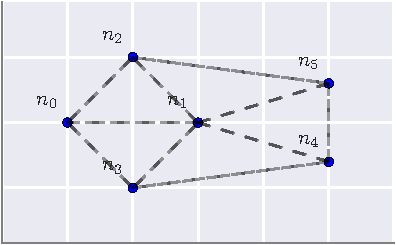
\includegraphics[width=0.45\textwidth]{img/s1_layout.pdf}
  \caption{Initial Scenario Topology, with nodes spaced an average of 100m apart}
  \label{fig:s1_layout}
\end{figure}

Guo demonstrated that when compared against OTMF and Beta trust assessment, MTFM provided increased variation in trust assessment over time, providing more information about the nodes behaviour than simply the probabilistic nature of packet delivery. 
It was also demonstrated that this MTFM valuation was stochastically stable for varying mobilities.
Further, by dynamically weighting the metrics used in MTFM, it was shown that the trust assessments could be used to identify the style of attack / selfishness being performed within the network and by who

We present a corrolary method to investigate and apply this work to the Marine MANET field.

\subsection{Simulation Background}

Simulations were conducted using a Python based agent simulation framework based on SimPy\cite{Mueller2003SimPy}, with a network stack built upon the AUVNetSim stack\cite{Miquel2008}, with transmission parameters (Table \ref{tab:sysconstraints}) taken from and validated against \cite{Stojanovic2007} and \cite{Stefanov2011}.

Given the differences in delay and propagation between RF and marine networks, it is natural that the same application rates (e.g. packet emission rates or throughput) and node separations should not be assumed to be equivalently performant.
Therefore, we first characterise an operational zone of performance within which the network can operate normally.

\begin{table}[h]
  \caption{Comparison of system model constraints as applied between Terrestrial and Marine communications} \label{tab:sysconstraints}
  \begin{center}
    \setlength{\tabcolsep}{8pt}
    \begin{tabular}{lccc}
      \toprule
      Parameter & Unit & Terrestrial & Marine \\
      \midrule
      Simulated Duration & $s$ & 300 & 36000\\
      Simulated Area & $km^2$ & 0.7 & Various \\
      Transmission Range & $km$ & 0.25 & 1.5 \\
      Number of Nodes & & 6 & 6 \\
      Physical Layer & & RF(802.11) & Acoustic\\
      Propagation Speed& $m/s$ & $3\times10^8$ & 1490\\
      Center Frequency& $Hz$ & $2.6\times10^9$ & $2 \times 10^3$ \\
      Bandwidth& $Hz$ & $22\times10^6$ & $10^3$\\
      MAC Type & & CSMA/CA & CSMA/CA\\
      Routing Protocol & & DSDV & FBR \\
      Mobility & & Various & Various \\
      Max Speed & $ms^{-1}$ & 5 & 2.4 \\
      Data Rate & $bps$ & $10^6$ & 240 \\
      Burst Counts & & 10 & 1 \\
      Packet Size & bits & 4096 &  9600 \\
      Destination Selection & & Random & Random\\
      Single Transmission Duration & $s$ & 10 & 32 \\
      Single Transmission Size & bits & $10^7$ & $9600$ \\
      \bottomrule
    \end{tabular}
    \setlength{\tabcolsep}{6pt}
  \end{center}
\end{table}


\subsection{Scaling Considerations between Terrestrial and Underwater Environments}

In this section we characterise the simulated communications environment, establishing an optimal packet emission rate for comparison against \cite{Guo11}.

We establish a appropriate safe operating zone for marine communications by looking at the communications rate and physical distribution factors together across the four presented scenarios.
In scaling the physical distribution of the nodes, we also scale the environment in which the nodes are restricted to, which has a significant impact on the number of potential runtime topologies, wich nodes getting 'lost' in the far corner of an envionment for example. 
From Table~\ref{tab:sysconstraints}, the operating transmission range of acoustic is $\approx 6$ times further than 802.11, indicating that a suitable operating environment will have an area $\approx \sqrt{6}$ times the area of the 802.11 case.
Therefore, a reasonable experimental range would have an upper bound of performance around this scaling factor, where nodes are approximately 400$m$ apart. 
We select throughput and end to end delay as the targeted aspects of the networks performance to optimise against.
The raw results of these two metrics in the four mobility scenarios are shown in Fig.~\ref{fig:scenario_throughputs_plain}.
We take the ratio of throughput per second of delay as a combined proxy for this optimisation. $T/d$, shown in Fig.~\ref{fig:scenario_throughputratios_2d}.

It is clear that as the separation is increased, the emission rate at which the network becomes saturated reduces, reducing the overall throughput. 
This throughput degredation is tightly coupled with the mobility scenario.
For instance, in Fig.~\ref{fig:throughput_static}, where all nodes are static, we do not see significant drops in saturation rates until we approach 800m, nearly double our estimate. 
Compare that with Figs.~\ref{fig:throughput_allbut1} and ~\ref{fig:throughput_all_mobile}, where the majority or all the nodes are randomly walking, and the saturtion point collapses from 0.0258pps at 300m to 0.015pps at 400m.\todo{Add in Table here for delay characteristics too and talk about that, drawing the conclusion that 300 is better than 400 because you can increase the emmission rate!}
These results indicate that the best area to continue operating in for a variety of node separations is at 0.015pps, and that a reasonable position scaling is from 100m to 300m, beyond which communication becomes increasingly unstable, especially in terms of end to end delay.


\begin{figure}
\begin{subfigure}{.5\textwidth}
  \centering
  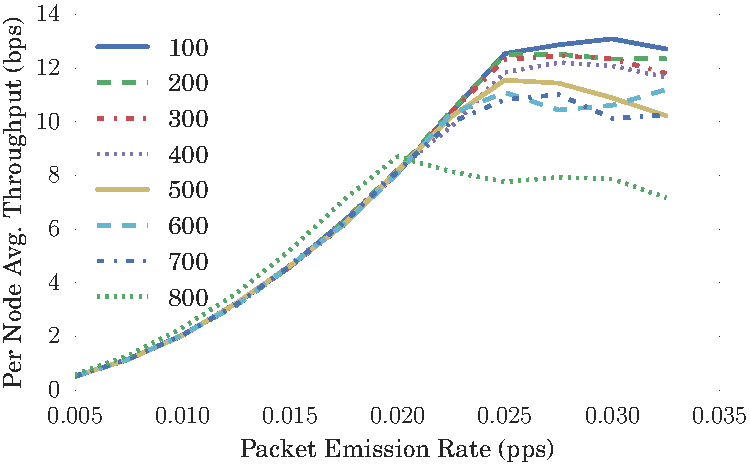
\includegraphics[width=.9\linewidth]{img/throughput_sep_lines_static.pdf}
  \caption{All Nodes Static}
  \label{fig:throughput_static}
\end{subfigure}%
\begin{subfigure}{.5\textwidth}
  \centering
  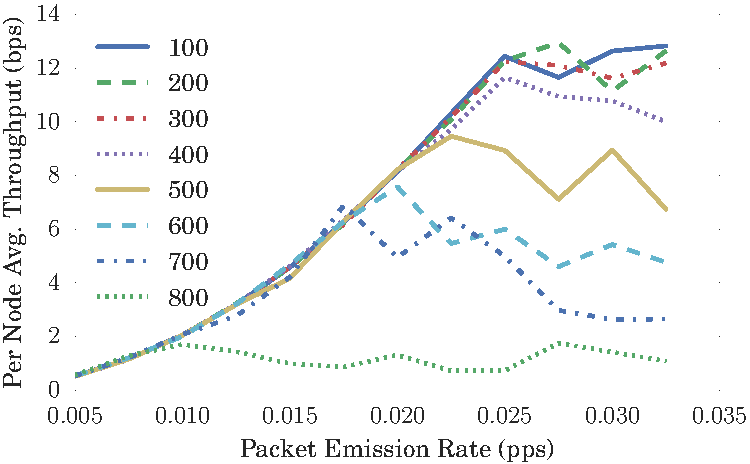
\includegraphics[width=.9\linewidth]{img/throughput_sep_lines_single_mobile.pdf}
  \caption{$n_1$ Random Walk}
  \label{fig:throughput_single_mobile}
\end{subfigure}
\begin{subfigure}{.5\textwidth}
\centering
  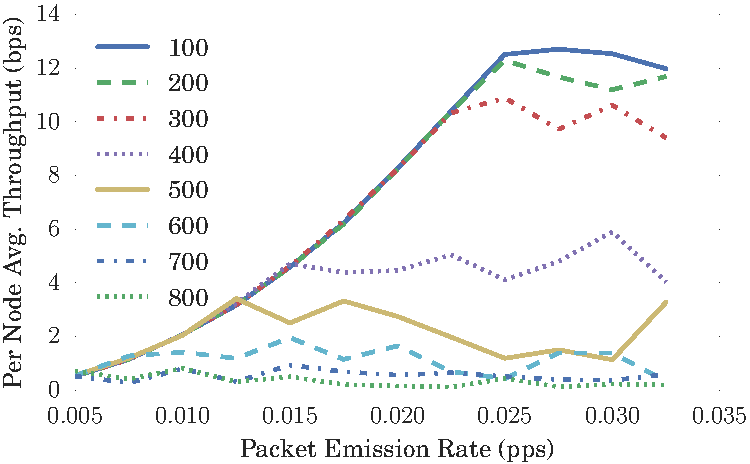
\includegraphics[width=.9\linewidth]{img/throughput_sep_lines_allbut1.pdf}
  \caption{All nodes but $n_1$ Random Walk}
  \label{fig:throughput_allbut1}
\end{subfigure}
\begin{subfigure}{.5\textwidth}
\centering
  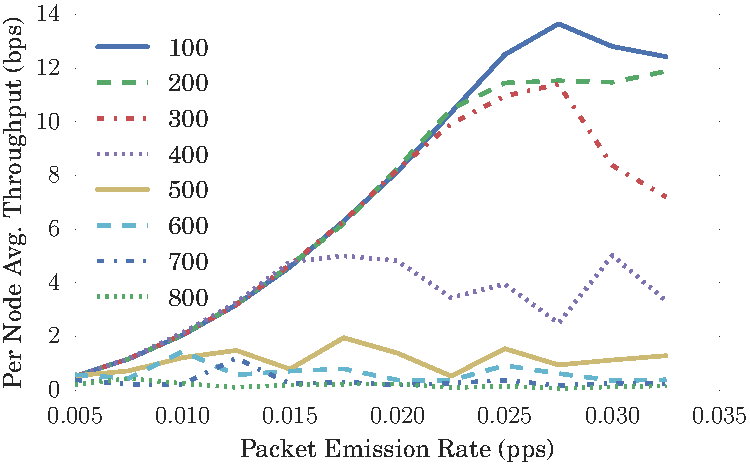
\includegraphics[width=.9\linewidth]{img/throughput_sep_lines_all_mobile.pdf}
  \caption{All Nodes Mobile}
  \label{fig:throughput_all_mobile}
\end{subfigure}
\caption{Throughput Characteristics for varying node separations across increasing packet emission rates}
\label{fig:scenario_throughputs_plain}
\end{figure}

\begin{figure}
\begin{subfigure}{.5\textwidth}
    \centering
  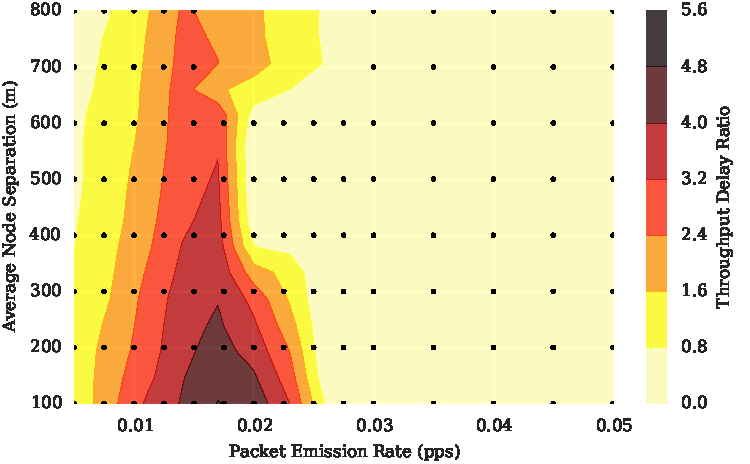
\includegraphics[width=.9\linewidth]{img/2d_ratio_static.pdf}
  \caption{All Nodes Static}
  \label{fig:throughput_static}
\end{subfigure}%
\begin{subfigure}{.5\textwidth}
  \centering
  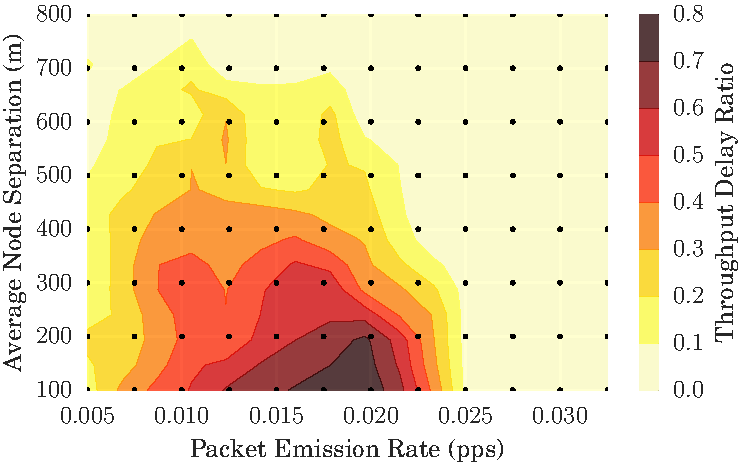
\includegraphics[width=.9\linewidth]{img/2d_ratio_single_mobile.pdf}
  \caption{$n_1$ Random Walk}
  \label{fig:throughput_single_mobile}
\end{subfigure}
\begin{subfigure}{.5\textwidth}
\centering
  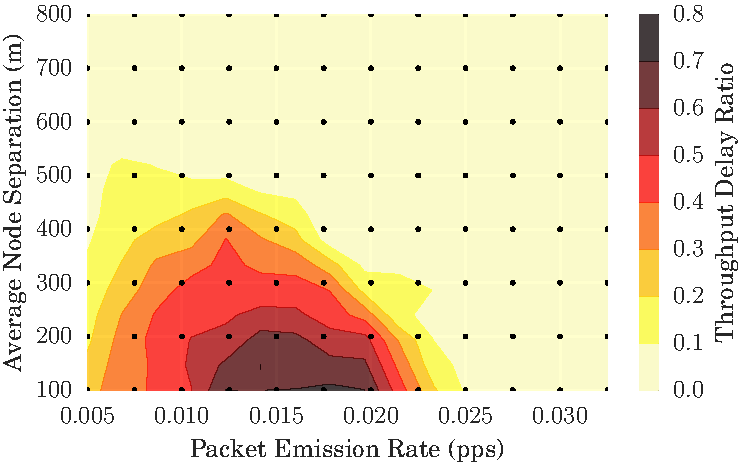
\includegraphics[width=.9\linewidth]{img/2d_ratio_allbut1.pdf}
  \caption{All nodes but $n_1$ Random Walk}
  \label{fig:throughput_allbut1}
\end{subfigure}
\begin{subfigure}{.5\textwidth}
\centering
  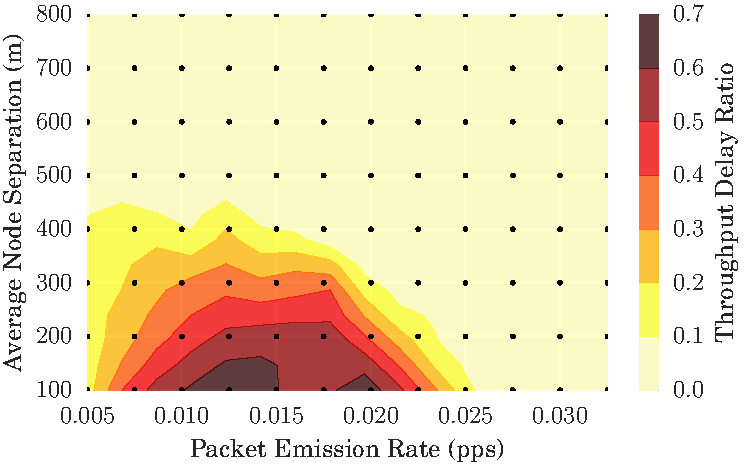
\includegraphics[width=.9\linewidth]{img/2d_ratio_all_mobile.pdf}
  \caption{All Nodes Mobile}
  \label{fig:throughput_all_mobile}
\end{subfigure}
\caption{Throughput/Delay Characteristics for varying node separations across increasing packet emission rates}
\label{fig:scenario_throughputratios_2d}
\end{figure}



\section{Trust}\label{sec:trustresultsanddiscussion}

Having established a safe operating range for comparison, at 300m separation with an emmission rate of 0.015pps, we proceed to repeat the scenarios presented in \cite{Guo11} in this simulated marine network. We select an assessment period of 10 mins within a 4 hour 'mission' to scale in comparison to the relative bitrates experienced (1Mbps vs $approx15$bps).

The particular factors under discussion are the relative performance of MTFM against OTMF and Beta with respect to statistical stability across mobilities and in responsiveness to changing network behaviour. 
We establish a similar result set by initially tracking the resultant trust values established by MTFM in each of the four mobility scenarios, shown in Fig.\ref{fig:trust_mobility}.
For simplicity, we are primarily concerned with the observational trust relationship between node 0 and node 1, i.e. $n_0$'s assessment of the trustworthiness of $n_1$, or $T_{1,0}$.
Some gropus use a reverse notation for trust, whereby $T_{1,0}$ would represent the trustworthiness of $n_1$ according to $n_0$; however, given the subjective nature of trustworthiness, it is more relatable to describe $T_{1,0}$ as ``The Trustworthiness of $n_1$ from the perspective of $n_0$. rather than an absolute statement on $n_1$'s trustworthiness.
We are also concerned with the opinions of $n_1$ provided to $n_0$ by other nodes, where ${T_{1,2},T_{1,2}$ and ${T_{1,2},T_{1,2}$ denote the sets of recommendation and indirect trust assessments respectively.
Also included are a set of aggregate assessments; $T_{1,\text{avg}}$, the flat average of direct trust assessments of $n_1$, $T_{1,\text{Net}}$, an aggregate that weights assessments according to the network topology from \eqref{eq:networkeffects}, and $T_{1,\text{MTFM}}$, the final MTFM trust assessment value based on both network topology and whitenisation from \eqref{eq:whitenization}.


From Fig.~\ref{fig:trust_static}, the generated trust values utilising the topology information ($T_{1,\text{Net}},T_{1,\text{MTFM}}$) display a greatly decreased variation than those of the individual subjective observations.

\begin{figure}
\begin{subfigure}{.5\textwidth}
  \centering
  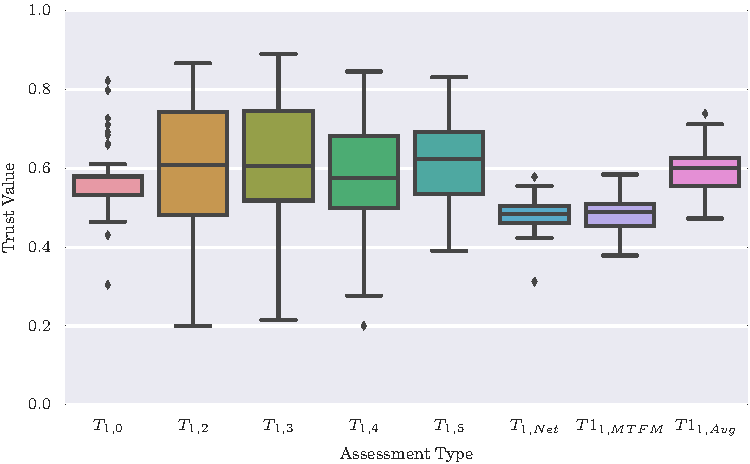
\includegraphics[width=.8\linewidth]{img/trust_bella_static.pdf}
  \caption{All Nodes Static}
  \label{fig:trust_static}
\end{subfigure}%
\begin{subfigure}{.5\textwidth}
  \centering
  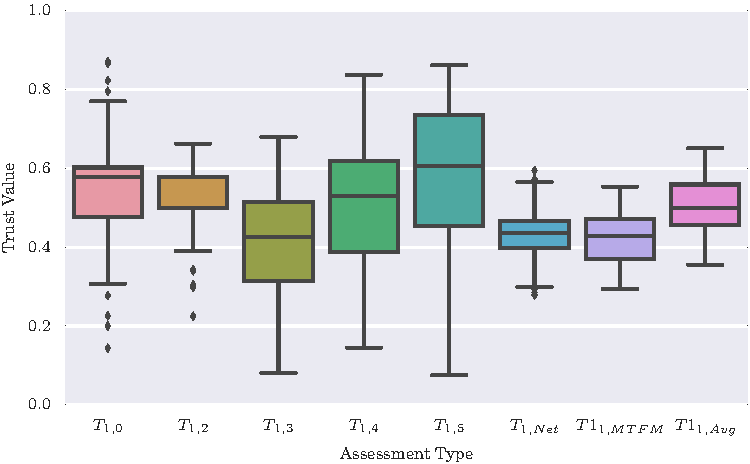
\includegraphics[width=.8\linewidth]{img/trust_bella_single_mobile.pdf}
  \caption{$n_1$ Randomly Walking}
  \label{fig:trust_single}
\end{subfigure}
\begin{subfigure}{.5\textwidth}
\centering
  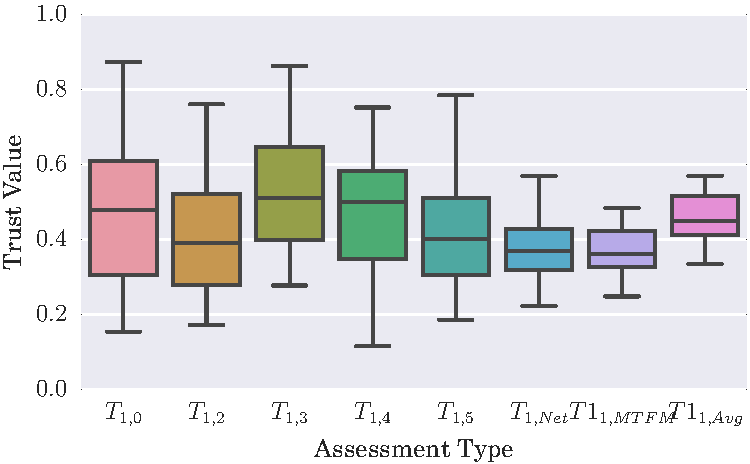
\includegraphics[width=.8\linewidth]{img/trust_bella_allbut1_mobile.pdf}
  \caption{All Nodes but $n_1$ Randomly Walking}
  \label{fig:trust_allbut1}
\end{subfigure}
\begin{subfigure}{.5\textwidth}
\centering
  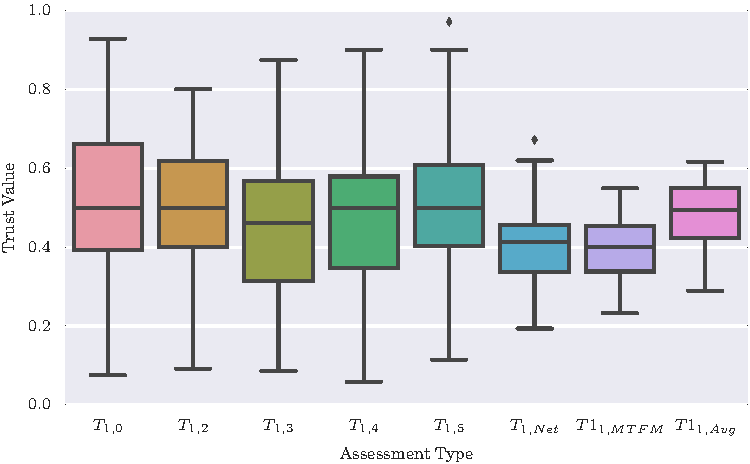
\includegraphics[width=.8\linewidth]{img/trust_bella_all_mobile.pdf}
  \caption{All Nodes Randomly Walking}
  \label{fig:trust_all_mobile}
\end{subfigure}
\caption{MTFM Trust assessments for varying mobility options}
\label{fig:trust_mobility}
\end{figure}

\begin{figure}
\begin{subfigure}{.5\textwidth}
  \centering
  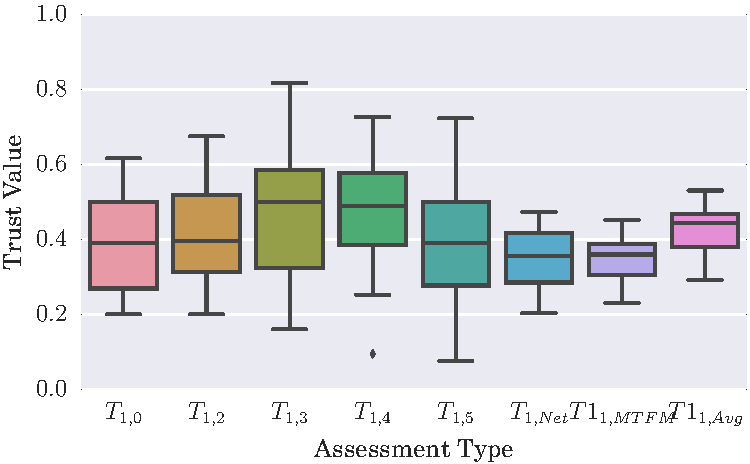
\includegraphics[width=.8\linewidth]{img/trust_bella_static_selfish.pdf}
  \caption{All Nodes Static}
  \label{fig:trust_static}
\end{subfigure}%
\begin{subfigure}{.5\textwidth}
  \centering
  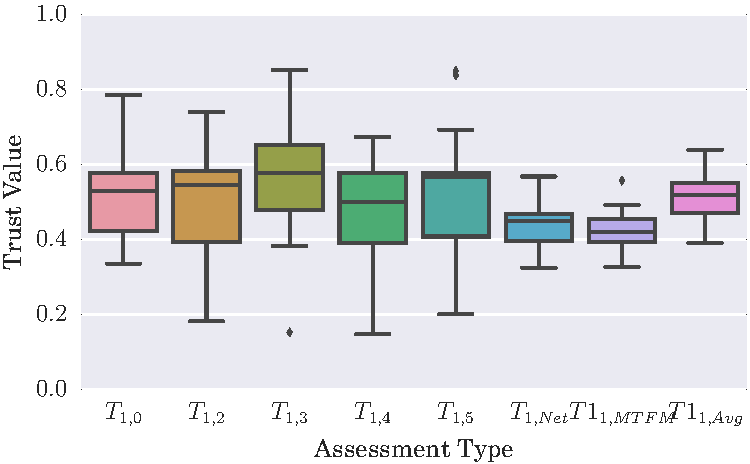
\includegraphics[width=.8\linewidth]{img/trust_bella_single_mobile_selfish.pdf}
  \caption{$n_1$ Randomly Walking}
  \label{fig:trust_single}
\end{subfigure}
\begin{subfigure}{.5\textwidth}
\centering
  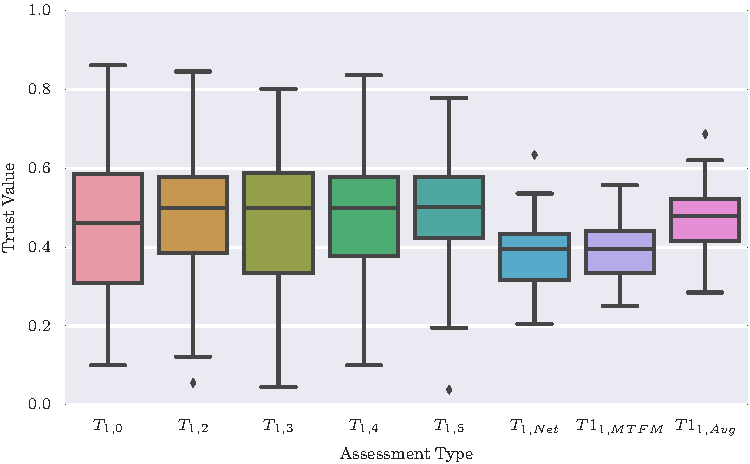
\includegraphics[width=.8\linewidth]{img/trust_bella_allbut1_mobile_selfish.pdf}
  \caption{All Nodes but $n_1$ Randomly Walking}
  \label{fig:trust_allbut1}
\end{subfigure}
\begin{subfigure}{.5\textwidth}
\centering
  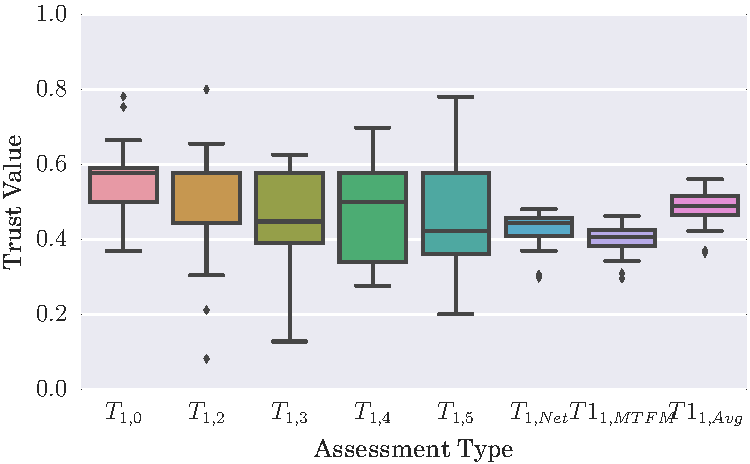
\includegraphics[width=.8\linewidth]{img/trust_bella_all_mobile_selfish.pdf}
  \caption{All Nodes Randomly Walking}
  \label{fig:trust_all_mobile}
\end{subfigure}
\caption{MTFM Trust assessments for varying mobility options}
\label{fig:trust_mobility}
\end{figure}

\begin{figure}
\begin{subfigure}{\textwidth}
  \centering
  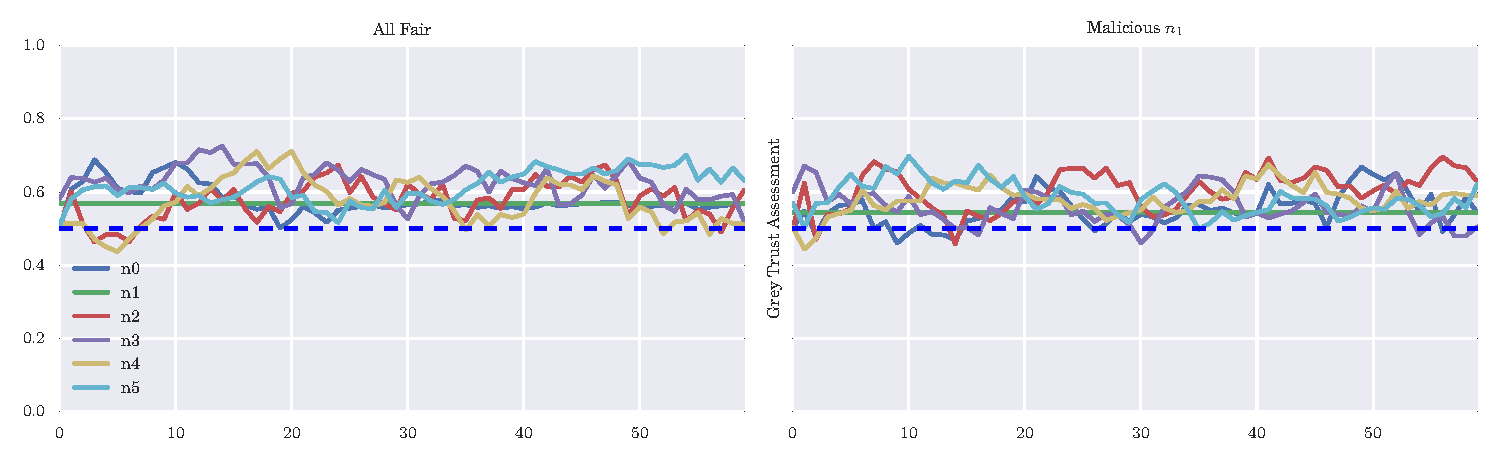
\includegraphics[width=.8\linewidth]{img/grey_trust_bella_static_joint.pdf}
  \caption{All Nodes Static}
  \label{fig:grey_trust_static}
\end{subfigure}
\begin{subfigure}{\textwidth}
  \centering
  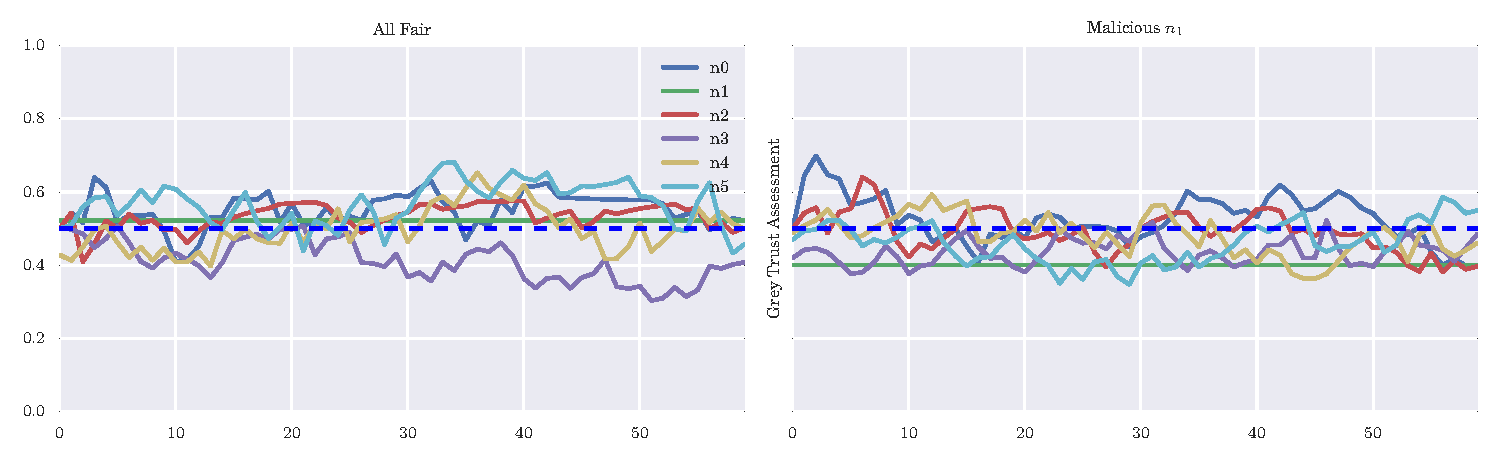
\includegraphics[width=.8\linewidth]{img/grey_trust_bella_single_mobile_joint.pdf}
  \caption{$n_1$ Randomly Walking}
  \label{fig:grey_trust_single}
\end{subfigure}
\begin{subfigure}{\textwidth}
\centering
  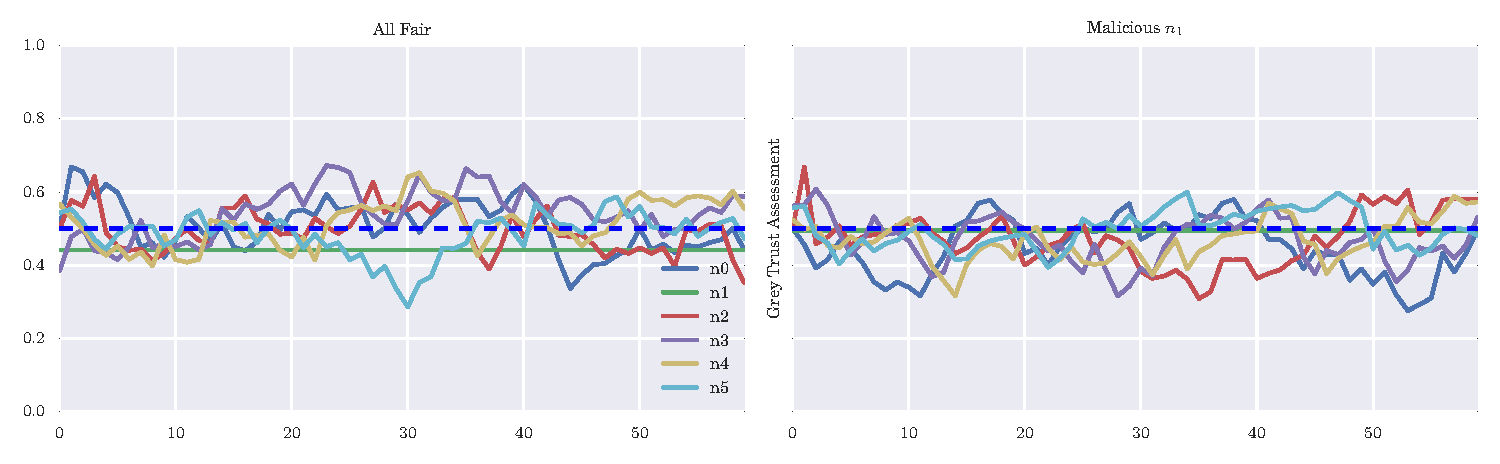
\includegraphics[width=.8\linewidth]{img/grey_trust_bella_allbut1_mobile_joint.pdf}
  \caption{All Nodes but $n_1$ Randomly Walking}
  \label{fig:grey_trust_allbut1}
\end{subfigure}
\begin{subfigure}{\textwidth}
\centering
  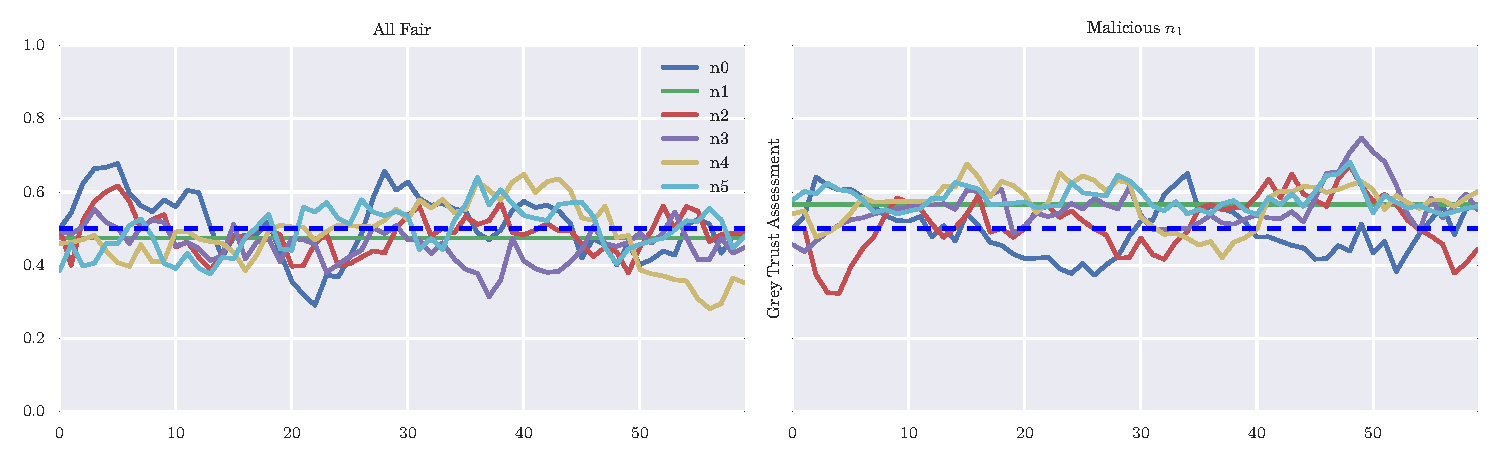
\includegraphics[width=.8\linewidth]{img/grey_trust_bella_all_mobile_joint.pdf}
  \caption{All Nodes Randomly Walking}
  \label{fig:grey_trust_all_mobile}
\end{subfigure}
\caption{MTFM Trust time varying assessments for of $n1$ varying mobility options}
\label{fig:trust_mobility}
\end{figure}

\begin{figure}
\begin{subfigure}{\textwidth}
  \centering
  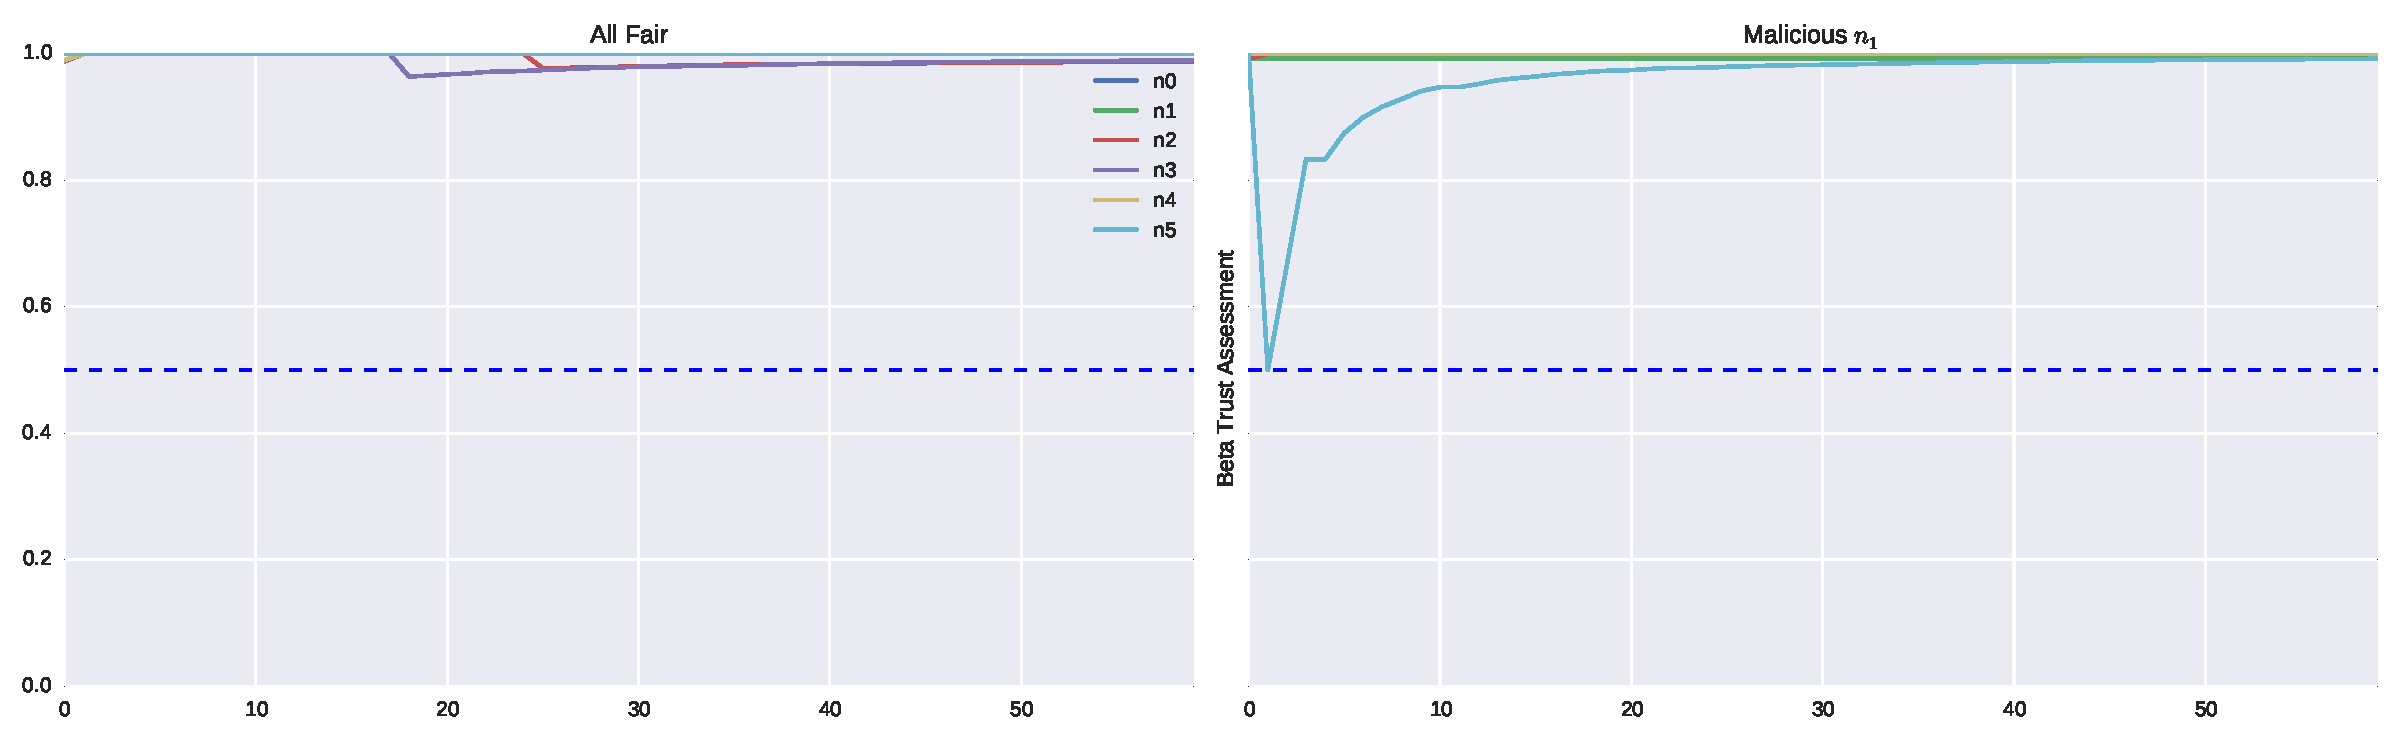
\includegraphics[width=.8\linewidth]{img/beta_trust_bella_static_joint.pdf}
  \caption{All Nodes Static}
  \label{fig:beta_trust_static}
\end{subfigure}
\begin{subfigure}{\textwidth}
  \centering
  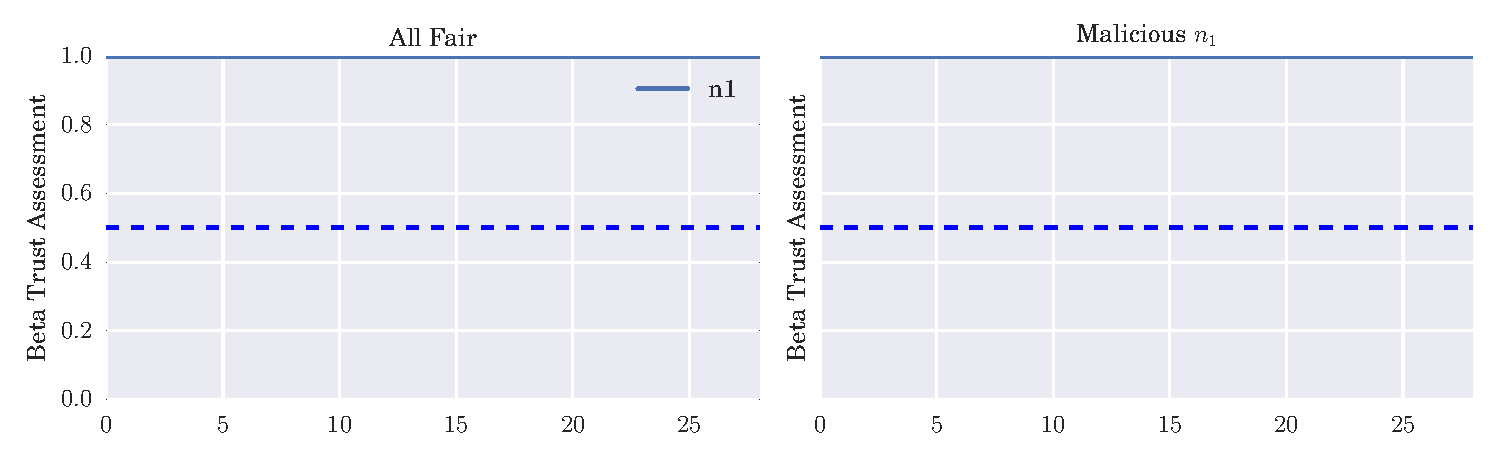
\includegraphics[width=.8\linewidth]{img/beta_trust_bella_single_mobile_joint.pdf}
  \caption{$n_1$ Randomly Walking}
  \label{fig:beta_trust_single}
\end{subfigure}
\begin{subfigure}{\textwidth}
\centering
  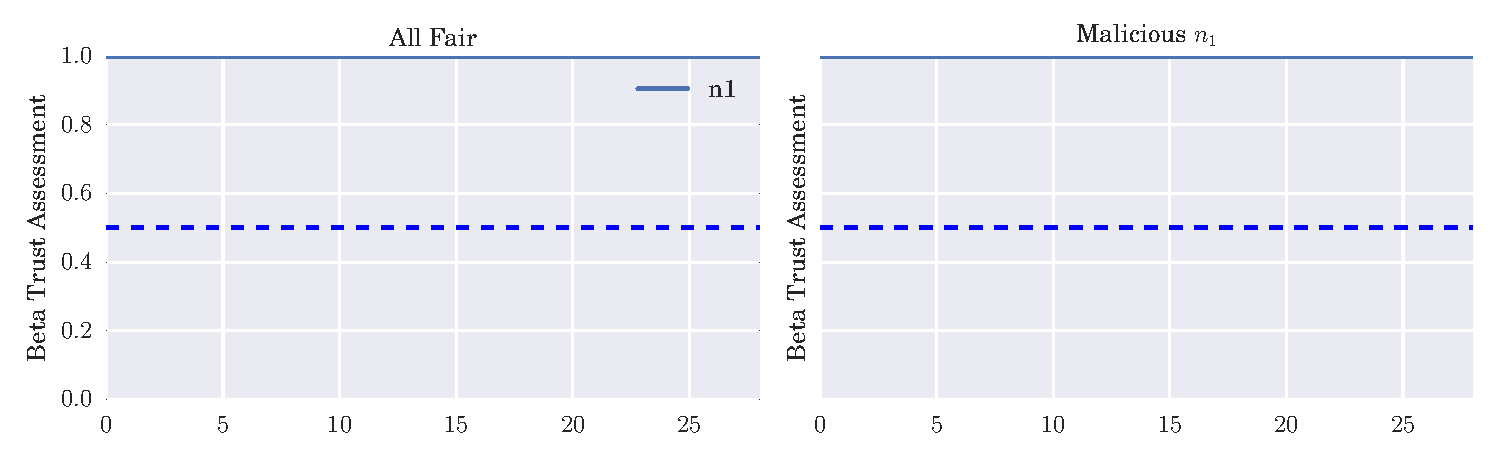
\includegraphics[width=.8\linewidth]{img/beta_trust_bella_allbut1_mobile_joint.pdf}
  \caption{All Nodes but $n_1$ Randomly Walking}
  \label{fig:beta_trust_allbut1}
\end{subfigure}
\begin{subfigure}{\textwidth}
\centering
  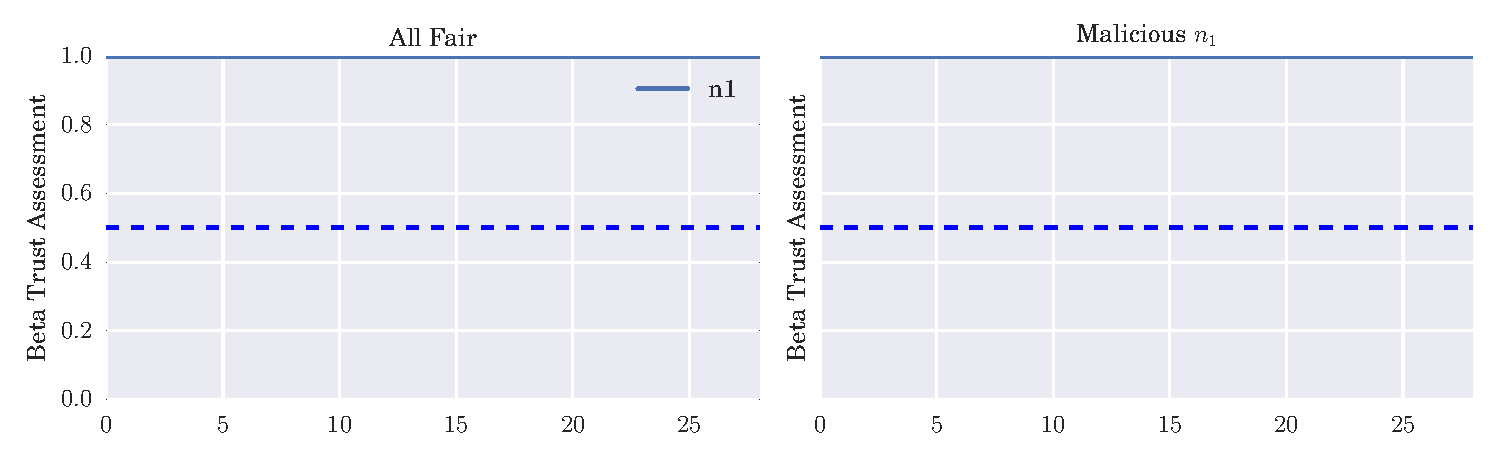
\includegraphics[width=.8\linewidth]{img/beta_trust_bella_all_mobile_joint.pdf}
  \caption{All Nodes Randomly Walking}
  \label{fig:beta_trust_all_mobile}
\end{subfigure}
\caption{Beta Trust time varying assessments for of $n1$ varying mobility options}
\label{fig:trust_mobility}
\end{figure}

\subsection{Metric Selection}

Initially, all the available metrics (transmitted and received throughput, delay, received signal strength, transmitted power, and packet loss rate) were utilised for Grey assessment. 
In context of Grey Relational Coefficient generation \eqref{eq:grc}, the best sequence $g$ was selected using the lowest PLR, delay, and recieved and transmitted power, with the highest throughputs, with the worst sequence, $b$ selected as the inverse of these.

\subsection{Weight Generation}

For an arbitrary metric weight vector $H$, where the metric $m_j$ is emphasised as being twice as important as the other metrics, we form an initial weighting vector $H' = [1,1,1,1,2,1]$ for $j=4$ for example. We then scale that vector $H'$ such that $\sum H = 1$ by $H= \frac{2 H'}{\max{H'}\times \sum H'}$.

Using this process we generate an emphasis matrix $\mathbf{E}$ consisting of a row vector $\mathbf{H}_j$ for each metric where additional emphasis is weighted on this metric, allowing a comparative analysis 

\begin{figure}
\begin{subfigure}{0.5\textwidth}
  \centering
  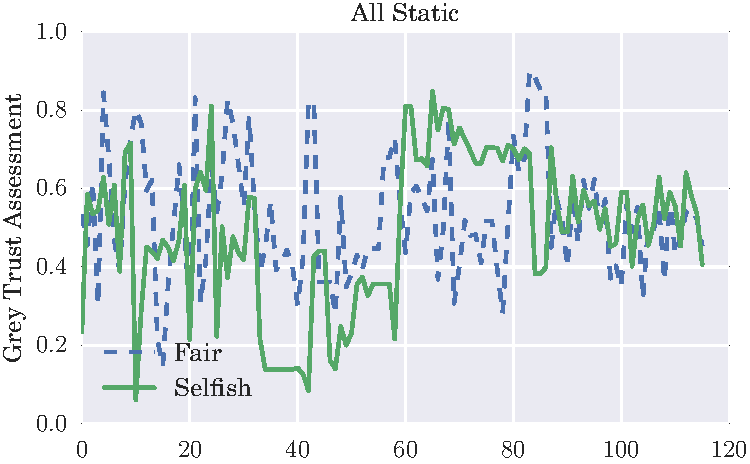
\includegraphics[width=.8\linewidth]{img/trust_bella_static_even_SelfishTargetSelection.pdf}
  \caption{All Metrics Evenly Weighted}
  \label{fig:beta_trust_static}
\end{subfigure}
\begin{subfigure}{0.5\textwidth}
  \centering
  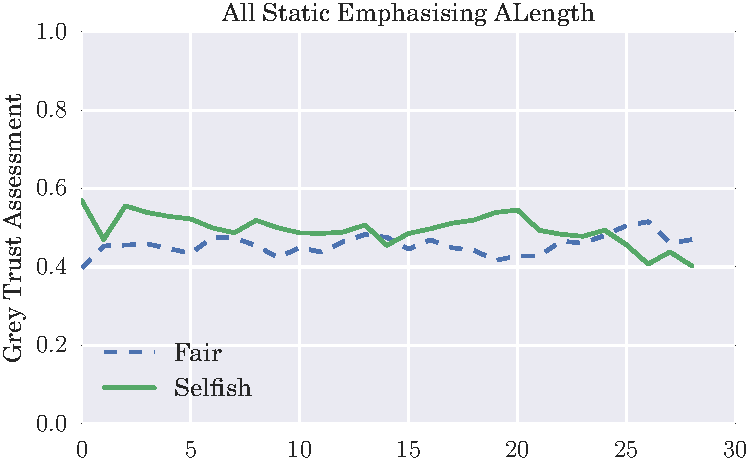
\includegraphics[width=.8\linewidth]{img/trust_bella_static_emph_ALength_SelfishTargetSelection.pdf}
  \caption{Average Packet Length Emphasised}
  \label{fig:beta_trust_single}
\end{subfigure}
\begin{subfigure}{0.5\textwidth}
  \centering
  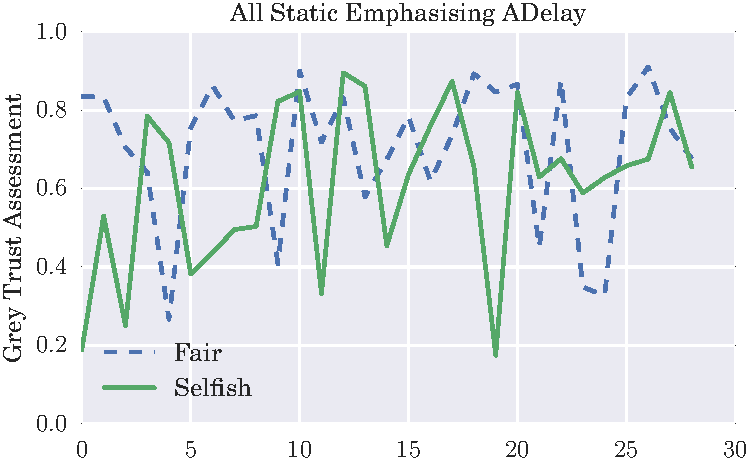
\includegraphics[width=.8\linewidth]{img/trust_bella_static_emph_ADelay_SelfishTargetSelection.pdf}
  \caption{Delay Emphasised}
  \label{fig:beta_trust_single}
\end{subfigure}
\begin{subfigure}{0.5\textwidth}
\centering
  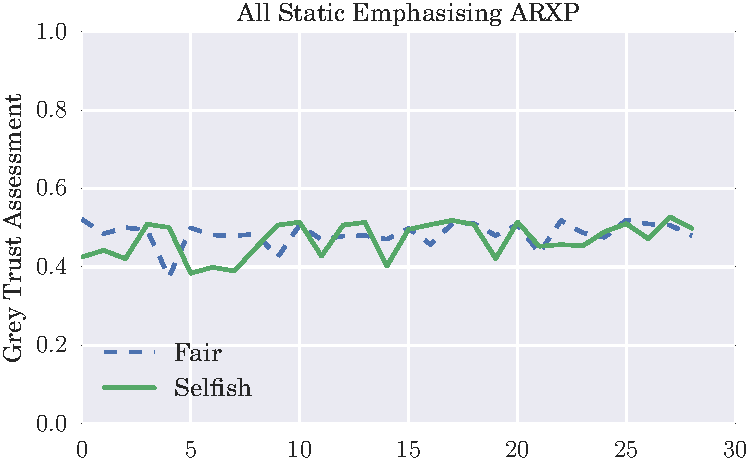
\includegraphics[width=.8\linewidth]{img/trust_bella_static_emph_ARXP_SelfishTargetSelection.pdf}
  \caption{Received Power Emphasised}
  \label{fig:beta_trust_allbut1}
\end{subfigure}
\begin{subfigure}{0.5\textwidth}
\centering
  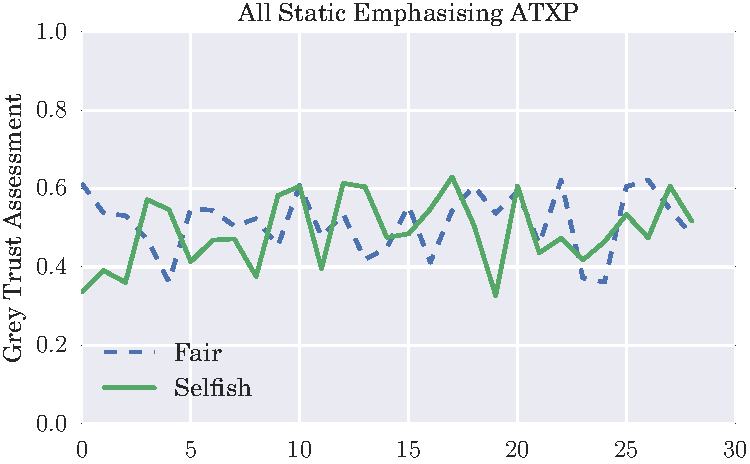
\includegraphics[width=.8\linewidth]{img/trust_bella_static_emph_ATXP_SelfishTargetSelection.pdf}
  \caption{Transmitted Power Emphasised}
  \label{fig:beta_trust_all_mobile}
\end{subfigure}
\begin{subfigure}{0.5\textwidth}
\centering
  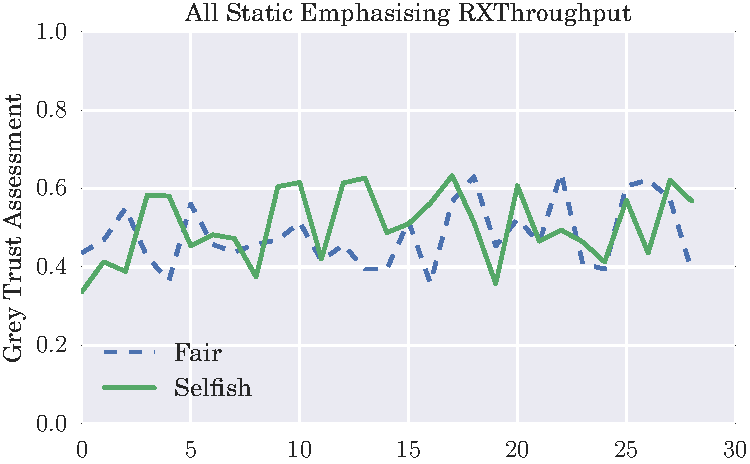
\includegraphics[width=.8\linewidth]{img/trust_bella_static_emph_RXThroughput_SelfishTargetSelection.pdf}
  \caption{Received Throughput}
  \label{fig:beta_trust_all_mobile}
\end{subfigure}
\begin{subfigure}{0.5\textwidth}
\centering
  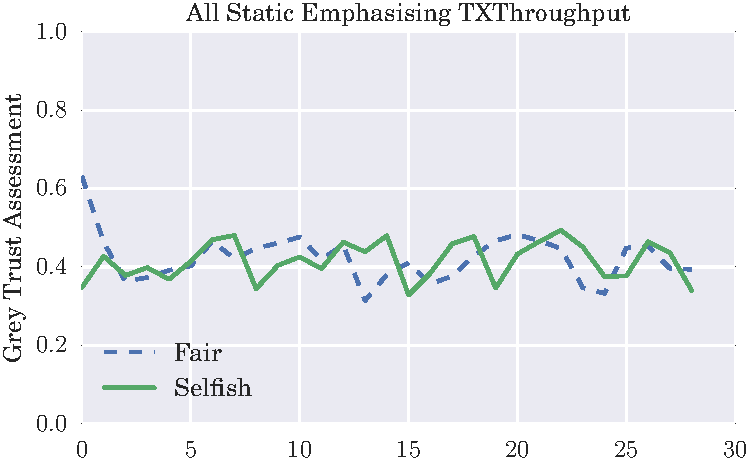
\includegraphics[width=.8\linewidth]{img/trust_bella_static_emph_TXThroughput_SelfishTargetSelection.pdf}
  \caption{Transmitted Throughput}
  \label{fig:beta_trust_all_mobile}
\end{subfigure}
\begin{subfigure}{0.5\textwidth}
\centering
  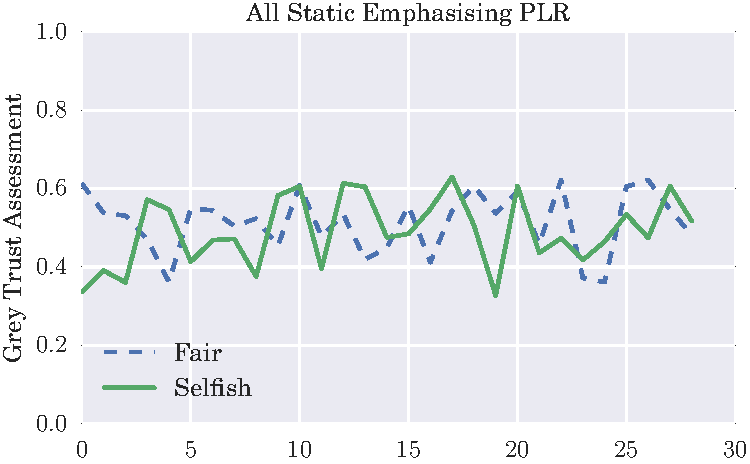
\includegraphics[width=.8\linewidth]{img/trust_bella_static_emph_PLR_SelfishTargetSelection.pdf}
  \caption{PLR Emphasised}
  \label{fig:beta_trust_all_mobile}
\end{subfigure}
\caption{$T_{1,0}$ in the Static case for the Selfish Selection behaviour}
\label{fig:trust_mobility}
\end{figure}

\begin{figure}
\begin{subfigure}{0.5\textwidth}
  \centering
  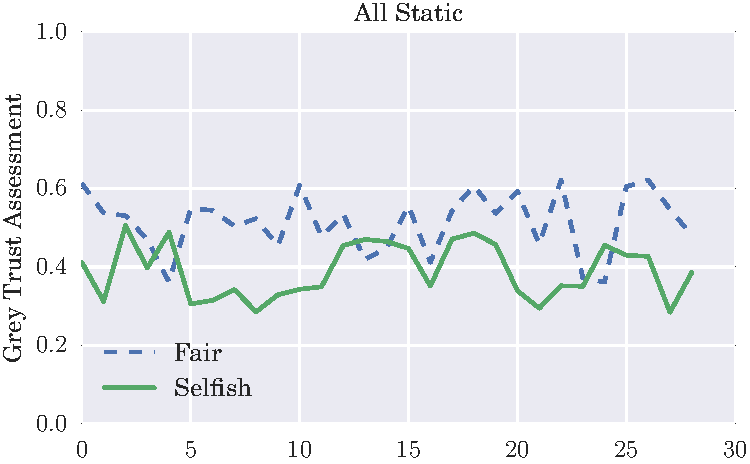
\includegraphics[width=.8\linewidth]{img/trust_bella_static_even_BadMouthingPowerControl.pdf}
  \caption{All Metrics Evenly Weighted}
  \label{fig:beta_trust_static}
\end{subfigure}
\begin{subfigure}{0.5\textwidth}
  \centering
  \includegraphics[width=.8\linewidth]{img/trust_bella_static_emph_ALength_BadMouthingPowerControl.pdf}
  \caption{Average Packet Length Emphasised}
  \label{fig:beta_trust_single}
\end{subfigure}
\begin{subfigure}{0.5\textwidth}
  \centering
  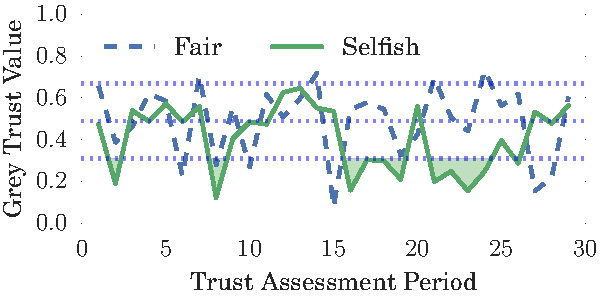
\includegraphics[width=.8\linewidth]{img/trust_bella_static_emph_ADelay_BadMouthingPowerControl.pdf}
  \caption{Delay Emphasised}
  \label{fig:beta_trust_single}
\end{subfigure}
\begin{subfigure}{0.5\textwidth}
\centering
  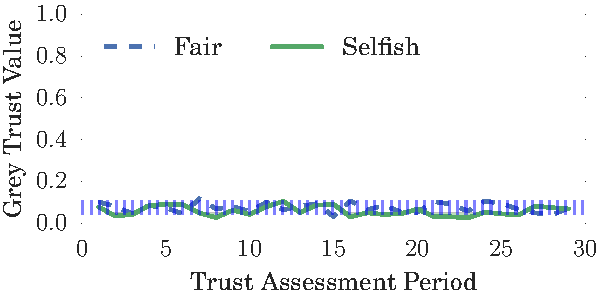
\includegraphics[width=.8\linewidth]{img/trust_bella_static_emph_ARXP_BadMouthingPowerControl.pdf}
  \caption{Received Power Emphasised}
  \label{fig:beta_trust_allbut1}
\end{subfigure}
\begin{subfigure}{0.5\textwidth}
\centering
  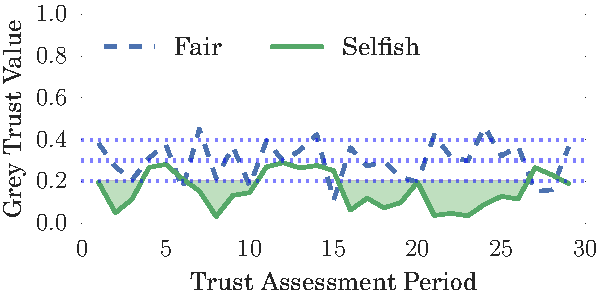
\includegraphics[width=.8\linewidth]{img/trust_bella_static_emph_ATXP_BadMouthingPowerControl.pdf}
  \caption{Transmitted Power Emphasised}
  \label{fig:beta_trust_all_mobile}
\end{subfigure}
\begin{subfigure}{0.5\textwidth}
\centering
  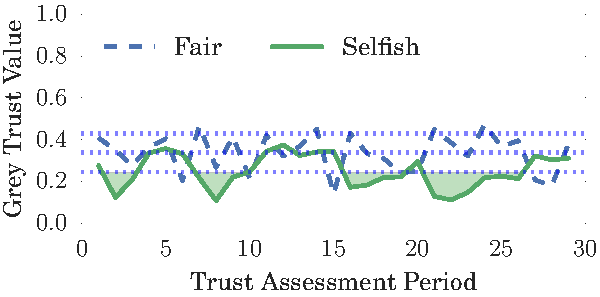
\includegraphics[width=.8\linewidth]{img/trust_bella_static_emph_RXThroughput_BadMouthingPowerControl.pdf}
  \caption{Received Throughput}
  \label{fig:beta_trust_all_mobile}
\end{subfigure}
\begin{subfigure}{0.5\textwidth}
\centering
  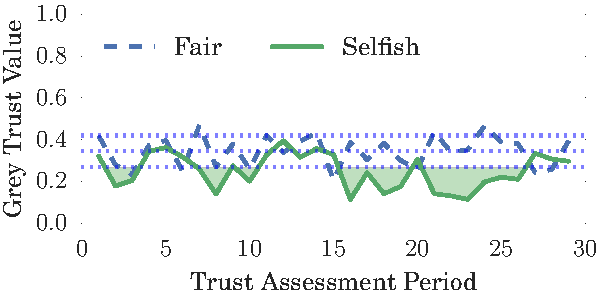
\includegraphics[width=.8\linewidth]{img/trust_bella_static_emph_TXThroughput_BadMouthingPowerControl.pdf}
  \caption{Transmitted Throughput}
  \label{fig:beta_trust_all_mobile}
\end{subfigure}
\begin{subfigure}{0.5\textwidth}
\centering
  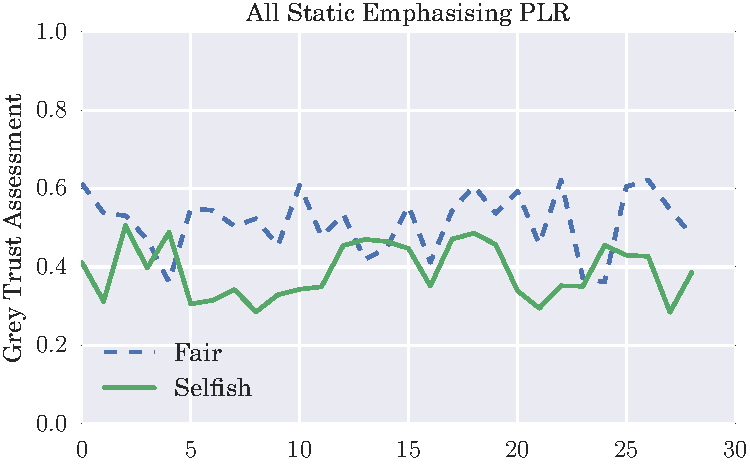
\includegraphics[width=.8\linewidth]{img/trust_bella_static_emph_PLR_BadMouthingPowerControl.pdf}
  \caption{PLR Emphasised}
  \label{fig:beta_trust_all_mobile}
\end{subfigure}
\caption{$T_{1,0}$ in the Static case for the Bad Mouthing Power Control behaviour}
\label{fig:trust_mobility}
\end{figure}





\subsection{Comparison to OTMF and Beta}

The same experiments were also performed utilising OTMF and Beta assessment as well as MTFM, providing like-for-like comparison of assessment at runtime.

It is important to note a distinction between the expectations of MTFM compared to other trust assessment frameworks; it is primarily concerned with the detection and identification of malicious or mistaken behaviours, and is relativistic in it's operation.
That is to day that under Grey Theory, agents are compared against the worst current performances across various metrics and graded against them.
OTMF and Beta in comparison are absolutist in their approach, and do not factor in a comparative metric for assessment; in the Bayesian book, you are good or bad regardless of what everyone else is doing. 
This relativistic vs absolutist differential is particularly stark when comparing mobility models. 

MTFM keeps a steady assessment that the node under assessment, $n_1$, is behaving ``OK'' regardless of mobility model. 
However, the network itself is most under strain with full mobility, with the routing topology changing every few minutes, requiring route advertisements and request overheads that contend the already valuable channel.

Another point to highlight is that computationally, MTFM is significantly more computationally intensive than the relatively simple Beta / OTMF implementation, and the repeated metric matrix reweighting required for reasonable behaviour detection.

As such, a hybrid system could be implemented, that used OTMF as a 'trigger' to detect potentially selfish or malicious behaviour, and allow MTMF to be triggered more slowly.

\subsection{Comparison under malicious behaviour}

Introducing a malicious actor into a trusted network with the aim to identifying the actor and the form of the malicious action is the driving force behind this work. 
Guo introduces a range of malicious actors, including modification of the packet loss rate of routing nodes and limiting throughput on a per-link basis as well as a selection of combined mis-behaviours. 

In all cases, the malicious node is $n_1$, the node that $n_1$ is ``attacking'' is $n0$, who is also the primary observer, e.g. the value of trust under assessment is $T_{0,1}$
\begin{itemize}
  \item \emph{Single Metric Misbehaviours}
    \begin{itemize}
      \item \emph{Packet Loss Rate}: $n_1$ selectivly denies $n_0$'s packets to reduce $n_0$'s apparrant PLR from the perspective of the rest of the network.
      \item \emph{Signal Strength}: $n_1$ increases it's standard operating signal strength for all nodes \emph{except} communications with $n_0$.
      \item \emph{Delay}: $n_1$ introduces artificial delays to it's communications with $n_0$
    \end{itemize}
\end{itemize}
Given that the established links are already heavily constrained, these heavy handed attacks can incidentally cripple the network.


\todo{All the 'programming' for this bit is done, it's just writing. Remember to highlight the relationships between delay/distance/trust and RSSI/PLR trust. Also remember to show the RTS ratio for the mobility case, highlighting that when the environment is significantly more dynamic and delay tolerant, beta/otmf fail to take that into account.}

\section{Conclusions and Future Work}
We have demonstrated that existing MANET Trust Management Frameworks cannot be directly applied to the contentious and dynamic underwater medium.
With significant delays (order from seconds to hours), a fading, refractive medium with varying propagation, the environment is simply not as predictable as classical MANET deployment environments. 

We presented a comparison scenario between trust establishment in Terrestrial MANET and in the underwater space, demonstrating that in order to have any reasonable expectation of performance, throughput and delay responses must be characterised before implementing trust in such environments. 

We demonstrated initial, unfiltered Grey Trust assessment utilising all the available metrics (transmitted and received throughput, delay, received signal strength, transmitted power, and packet loss rate)
Using the knowledge that in a 'fair' environment, trust assessments should be stable about 0.5, selected \todo{select metrics} THESE to continue. 

We have shown that existing frameworks are overly optimistic 
\todo{doesn't follow from rest of paragraph, needs to be expanded to explain the domain approach, possibly move back to 'future work' or something} \cite{Huang2010a} also raised the need for a more expanded view of trust but did so with a domain-partitioning approach rather than combining trust assessments from multiple domains within networks.

\subsubsection*{Acknowledgments.} The Authors would like to thanks the UK/FR DSTL PhD Programme for their support during this project.

\section{The References Section}\label{references}

\bibliographystyle{apalike}
%\bibliographystyle{amsplain} % UNCOMMENT BEFORE PUB!!!!!!!!!!!!!!!!!!!!!!!!!!!!!!!!!!!!!!!!!!!!!!1
\bibliography{refs}
% 
% \begin{thebibliography}{4}
% 
% \bibitem{jour} Smith, T.F., Waterman, M.S.: Identification of Common Molecular
% Subsequences. J. Mol. Biol. 147, 195--197 (1981)
% 
% \bibitem{lncschap} May, P., Ehrlich, H.C., Steinke, T.: ZIB Structure Prediction Pipeline:
% Composing a Complex Biological Workflow through Web Services. In: Nagel,
% W.E., Walter, W.V., Lehner, W. (eds.) Euro-Par 2006. LNCS, vol. 4128,
% pp. 1148--1158. Springer, Heidelberg (2006)
% 
% \bibitem{book} Foster, I., Kesselman, C.: The Grid: Blueprint for a New Computing
% Infrastructure. Morgan Kaufmann, San Francisco (1999)
% 
% \bibitem{proceeding1} Czajkowski, K., Fitzgerald, S., Foster, I., Kesselman, C.: Grid
% Information Services for Distributed Resource Sharing. In: 10th IEEE
% International Symposium on High Performance Distributed Computing, pp.
% 181--184. IEEE Press, New York (2001)
% 
% \bibitem{proceeding2} Foster, I., Kesselman, C., Nick, J., Tuecke, S.: The Physiology of the
% Grid: an Open Grid Services Architecture for Distributed Systems
% Integration. Technical report, Global Grid Forum (2002)
% 
% \bibitem{url} National Center for Biotechnology Information, \url{http://www.ncbi.nlm.nih.gov}
% 
% \end{thebibliography}

\listoftodos

\end{document}
